\documentclass[conference]{IEEEtran}
\IEEEoverridecommandlockouts
\usepackage{cite}
\usepackage{amsmath,amssymb,amsfonts}
\usepackage{booktabs}
\usepackage{enumitem}
\usepackage{tikz}
\usetikzlibrary{arrows.meta,positioning}

\newcommand{\sat}{\operatorname{sat}}
\newcommand{\diag}{\operatorname{diag}}

\begin{document}

\title{Quanser QBot Differential-Drive Robot:\\ Hardware Physics, Identification, Modelling, and the Complete Controller Suite\\
{\footnotesize Mathematical foundations for offline simulation, digital-twin, and hardware execution}}

\author{\IEEEauthorblockN{Gandhi Contreras}
\IEEEauthorblockA{\textit{Electrical and Computer Engineering}, New Mexico State University, Las Cruces, NM, USA \\ gandhico@nmsu.edu}}

\maketitle

\begin{abstract}
The QBot is a differential-drive ground robot. This paper develops its full mathematics: the battery--motor--wheel power chain, the rolling-contact physics that create the nonholonomic constraint, the sensing suite (wheel encoders, IMU, depth camera, LiDAR) with the dead-reckoning error-growth model that dictates the estimation architecture, identification of the kinematic and dynamic parameters, the unicycle and dynamic models with the tracking-error formulation, and the controller suite --- PID, LQR, LQG, backstepping, sliding mode, and NMPC --- stated with the structural fact that governs all of them: by Brockett's condition, no smooth time-invariant state feedback stabilizes a posture, so regulation and tracking are mathematically distinct problems on this platform.
\end{abstract}

\begin{IEEEkeywords}
Differential drive, nonholonomic systems, unicycle model, odometry, Brockett condition, backstepping, SMC, NMPC.
\end{IEEEkeywords}

%====================================================================
\section{Introduction}
Two independently driven wheels on a common axle (track $2b$, wheel radius $r_w$) plus a passive castor: forward speed and turn rate are commanded through the wheel speeds,
\begin{equation}
v = \frac{r_w}{2}\,(\omega_R + \omega_L),\qquad
\omega = \frac{r_w}{2b}\,(\omega_R - \omega_L).
\label{eq:diffmap}
\end{equation}
Pose $x_p = [X,\ Y,\ \psi]^{\!\top}$; the platform is underactuated in configuration (3 pose DOF, 2 inputs) but fully actuated in the $(v,\omega)$ velocity pair --- the structure from which everything below follows.

%====================================================================
\section{Hardware Physics}

\begin{figure*}[!t]
\centering
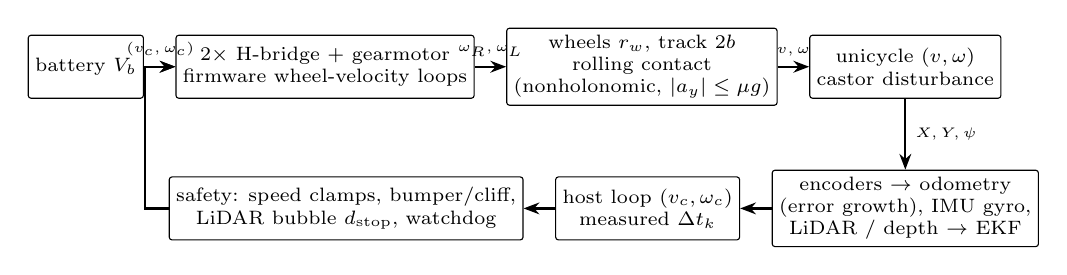
\begin{tikzpicture}[
  node distance=3mm and 4mm,
  blk/.style={draw, rounded corners=1pt, align=center, font=\scriptsize, inner sep=2.5pt, minimum height=8mm},
  lbl/.style={font=\tiny, align=center},
  arr/.style={-{Stealth[length=2mm]}, thick}
]

\node[blk] (bat) {battery $V_b$};
\node[blk, right=of bat] (hbr) {$2\times$ H-bridge + gearmotor\\ firmware wheel-velocity loops};
\node[blk, right=of hbr] (whl) {wheels $r_w$, track $2b$\\ rolling contact\\ (nonholonomic, $|a_y|\le\mu g$)};
\node[blk, right=of whl] (chas) {unicycle $(v,\omega)$\\ castor disturbance};
\node[blk, below=9mm of chas] (sens) {encoders $\to$ odometry\\ (error growth), IMU gyro,\\ LiDAR / depth $\to$ EKF};
\node[blk, left=of sens] (loop) {host loop $(v_c,\omega_c)$\\ measured $\Delta t_k$};
\node[blk, left=of loop] (safe) {safety: speed clamps, bumper/cliff,\\ LiDAR bubble $d_{\mathrm{stop}}$, watchdog};
\draw[arr] (bat) -- (hbr);
\draw[arr] (hbr) -- node[lbl, above] {$\omega_{R},\omega_{L}$} (whl);
\draw[arr] (whl) -- node[lbl, above] {$v,\omega$} (chas);
\draw[arr] (chas) -- node[lbl, right] {$X,Y,\psi$} (sens);
\draw[arr] (sens) -- (loop);
\draw[arr] (loop) -- (safe);
\draw[arr] (safe.west) -- ++(-3mm,0) |- node[lbl, pos=0.75, above] {$(v_c,\omega_c)$} (hbr.west);
\end{tikzpicture}
\caption{QBot signal chain: the rolling-contact constraint and odometry error growth dictate the estimation architecture; the LiDAR safety bubble scales with speed.}
\label{fig:chain}
\end{figure*}
\subsection{Power and drive}
Battery pack with loaded-voltage model $V_b = v_{\mathrm{oc}}(\mathrm{SoC}) - R_{\mathrm{int}}i_b$; per-wheel PWM H-bridges and DC gearmotors: $L_a\dot i + R_m i + k_e\omega_m = D V_b$, $\tau_m = k_t i$, through reduction $N_g$ to the wheel, so each wheel is first order in speed,
\begin{equation}
J_w\,\dot\omega_{R/L} = \eta_g N_g k_t\,i_{R/L} - b_w\,\omega_{R/L} - \tau_{\mathrm{load}},
\label{eq:wheel}
\end{equation}
with the load torque coupling both wheels through the chassis inertia. Most drive stacks close firmware velocity loops per wheel, making $(\omega_R^c, \omega_L^c)$ (equivalently $(v_c,\omega_c)$) the effective plant inputs with a first-order lag $\tau_v$ --- identified, not assumed. Manual-verified (QBot Platform): $12$~V $7$~Ah LiFePO$_4$ pack ($84$~Wh; $\sim$2~h at the typical $3.5$~A draw); per-motor transient current envelope from $4$~A for $6$~s down to $12$~A for $2$~s --- the current-clamp element of the safety envelope.

\subsection{Rolling contact: the nonholonomic constraint}
Rolling without slipping at each wheel imposes, at the chassis level, zero lateral velocity of the axle midpoint:
\begin{equation}
\dot X\sin\psi - \dot Y\cos\psi = 0 .
\label{eq:nonholo}
\end{equation}
This is real contact physics --- lateral tire stiffness against sliding friction --- valid below the friction limit $|a_y| \le \mu g$; violating it (aggressive turns, low-friction floors) invalidates the kinematic model and is the physical boundary of every design below. Castor dynamics add a small load-dependent yaw disturbance during reversals.

\subsection{Sensing and dead-reckoning physics}
Wheel encoders (quadrature, $N_{\mathrm{enc}}$ counts/rev at the motor, divided by $N_g$ at the wheel) integrate to odometry:
\begin{equation}
\hat X_{k+1} = \hat X_k + \Delta s_k\cos\hat\psi_k,\quad
\hat\psi_{k+1} = \hat\psi_k + \Delta\psi_k,
\end{equation}
with $\Delta s = \tfrac{r_w}{2}(\Delta\phi_R + \Delta\phi_L)$, $\Delta\psi = \tfrac{r_w}{2b}(\Delta\phi_R - \Delta\phi_L)$. The error physics: systematic errors (wheel-radius mismatch $\delta r$, track error $\delta b$) grow \emph{linearly} in distance and dominate heading drift; stochastic slip gives variance growing linearly in distance; and heading error injects position error $\propto$ distance $\times\ \sigma_\psi$ --- unbounded. Hence the estimation architecture: gyro-aided heading (IMU yaw rate, bias-corrected as on our other platforms) and exteroceptive correction (LiDAR scan matching / visual features) in an EKF; (QBot Platform: Leishen M10P 2-D LiDAR, $1680$ points/rev at $10$~Hz, $905$~nm Class~I eye-safe; Intel RealSense D435 RGB-D;) odometry alone is a prediction model, never a localization solution.

\subsection{Loop and safety}
Sampled loop with ZOH and measured-$\Delta t$ updates; safety: wheel-speed and acceleration clamps, tilt/cliff and bumper interlocks, LiDAR safety bubble (velocity-scaled stopping distance $d_{\mathrm{stop}} = v^2/2a_{\max} + v\,\tau_{\mathrm{delay}}$), watchdog, undervoltage return/stop.

%====================================================================
\section{Models}
\subsection{Unicycle kinematics}
\begin{equation}
\dot X = v\cos\psi,\qquad \dot Y = v\sin\psi,\qquad \dot\psi = \omega,
\label{eq:unicycle}
\end{equation}
with \eqref{eq:diffmap} mapping to wheels; inputs $(v,\omega)$ through the drive lags.

\subsection{Dynamic extension}
Applying the constrained Euler--Lagrange equations with \eqref{eq:nonholo} (Lagrange multiplier eliminated by projection onto the feasible distribution) gives
\begin{equation}
\bar M\begin{bmatrix}\dot v\\ \dot\omega\end{bmatrix} =
\begin{bmatrix}\frac{1}{r_w}(\tau_R + \tau_L) - F_{\mathrm{res}}\\[2pt]
\frac{b}{r_w}(\tau_R - \tau_L) - \tau_{\mathrm{res}}\end{bmatrix},\;\;
\bar M = \diag\!\bigl(m + \tfrac{2J_w}{r_w^2},\ I_z + \tfrac{2J_w b^2}{r_w^2}\bigr),
\label{eq:dyn}
\end{equation}
diagonal because the c.o.m. is on the axle (offset $d$ adds the coupling terms $m d\omega^2$, $m d\dot\omega$); $F_{\mathrm{res}}, \tau_{\mathrm{res}}$ collect rolling resistance and viscous plus smoothed-Coulomb friction, $b\,\dot q + \tau_c\tanh(\dot q/\epsilon)$ per channel.

\subsection{Tracking error model and the structural obstruction}
For a reference trajectory $(X_r, Y_r, \psi_r)$ with feasible $(v_r, \omega_r)$, the error in the body frame,
\begin{equation}
\begin{bmatrix}e_x\\ e_y\\ e_\psi\end{bmatrix} =
\begin{bmatrix}\cos\psi & \sin\psi & 0\\ -\sin\psi & \cos\psi & 0\\ 0&0&1\end{bmatrix}
\begin{bmatrix}X_r - X\\ Y_r - Y\\ \psi_r - \psi\end{bmatrix},
\end{equation}
obeys
\begin{equation}
\dot e_x = \omega e_y - v + v_r\cos e_\psi,\;\;
\dot e_y = -\omega e_x + v_r\sin e_\psi,\;\;
\dot e_\psi = \omega_r - \omega.
\label{eq:trackerr}
\end{equation}
Linearized about $e=0$ this is controllable \emph{iff} $v_r \neq 0$ or $\omega_r \neq 0$ (persistent motion). For the fixed posture ($v_r{=}\omega_r{=}0$), Brockett's necessary condition fails: \emph{no smooth time-invariant feedback stabilizes \eqref{eq:unicycle} to a point}; posture regulation requires time-varying, discontinuous, or switching laws (e.g., polar-coordinate control). Every controller below is therefore stated for tracking, with the posture case flagged where its law differs.

%====================================================================
\section{Identification}

\begin{figure}[!t]
\centering
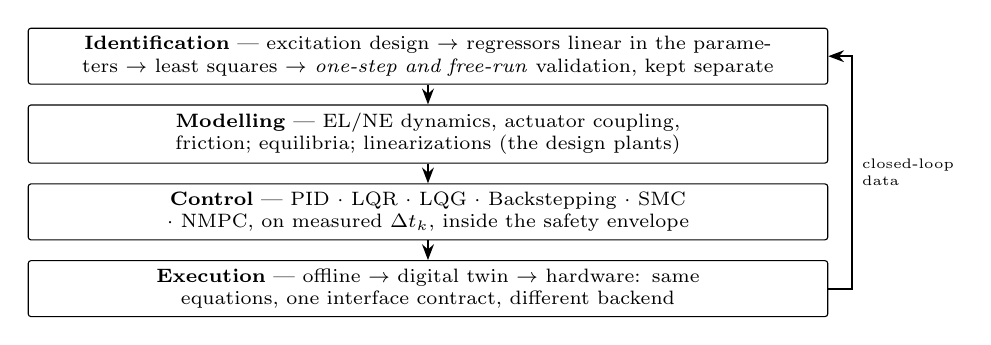
\begin{tikzpicture}[
  node distance=2.5mm,
  blk/.style={draw, rounded corners=1pt, align=center, font=\scriptsize, inner sep=3pt, text width=0.82\columnwidth},
  arr/.style={-{Stealth[length=2mm]}, thick}
]
\node[blk] (id) {\textbf{Identification} --- excitation design $\to$ regressors linear in the parameters $\to$ least squares $\to$ \emph{one-step and free-run} validation, kept separate};
\node[blk, below=of id] (mod) {\textbf{Modelling} --- EL/NE dynamics, actuator coupling, friction; equilibria; linearizations (the design plants)};
\node[blk, below=of mod] (ctl) {\textbf{Control} --- PID $\cdot$ LQR $\cdot$ LQG $\cdot$ Backstepping $\cdot$ SMC $\cdot$ NMPC, on measured $\Delta t_k$, inside the safety envelope};
\node[blk, below=of ctl] (exe) {\textbf{Execution} --- offline $\to$ digital twin $\to$ hardware: same equations, one interface contract, different backend};
\draw[arr] (id) -- (mod);
\draw[arr] (mod) -- (ctl);
\draw[arr] (ctl) -- (exe);
\draw[arr] (exe.east) -- ++(3mm,0) |- node[font=\tiny, pos=0.25, right, align=left] {closed-loop\\ data} (id.east);
\end{tikzpicture}
\caption{The workflow every platform in this series follows: identification feeds modelling, modelling feeds the controller suite, and all stages run unchanged across the three execution targets; closed-loop records return to identification.}
\label{fig:workflow}
\end{figure}
E1) \emph{drive lag}: wheel-speed steps against encoder rates, fit gain/$\tau_v$ per wheel; E2) \emph{kinematic calibration}: UMBmark-style square paths identify $\delta r$ (straight-line drift) and effective $b$ (turn scaling) --- linear least squares on the systematic-odometry model; E3) \emph{dynamics}: acceleration transients regress \eqref{eq:dyn}, linear in $(\bar M_{11}, \bar M_{22}, F_{\mathrm{res}}, \tau_{\mathrm{res}})$; E4) IMU gyro bias/noise by the stationary procedure common to our platforms; validation via held-out trajectories, odometry vs.\ ground truth, one-step and free-run reported separately.

%====================================================================
\section{Control Suite}
Inner wheel-velocity loops (firmware or PI, anti-windup at the PWM bound) receive $(v_c,\omega_c)$ from the outer laws below; all discrete updates on measured $\Delta t_k$.

\subsection{PID}
Heading-and-speed decomposition: $v_c$ = PI on along-track error (or profile feedforward $v_r$); $\omega_c = k_p e_\psi^{\mathrm{la}} + k_d\dot e_\psi$ on the look-ahead heading error $e_\psi^{\mathrm{la}} = \operatorname{atan2}(y_t, x_t)$ to a target point at distance $L_d$ (pure-pursuit geometry: $\omega_c = 2v\sin e_\psi^{\mathrm{la}}/L_d$ is the exact-arc special case). Derivatives from the shared filtered differentiator.

\subsection{LQR / LQG}
On the linearization of \eqref{eq:trackerr} about the moving reference,
\begin{equation}
A(t) = \begin{bmatrix}0&\omega_r&0\\ -\omega_r&0&v_r\\ 0&0&0\end{bmatrix},\qquad
B = \begin{bmatrix}1&0\\0&0\\0&1\end{bmatrix}\!\!\begin{array}{l}\scriptstyle(\delta v)\\ \\ \scriptstyle(\delta\omega)\end{array}
\end{equation}
gain-scheduled on $(v_r,\omega_r)$; $[\delta v,\ \delta\omega]^{\!\top} = -K_{\mathrm{lqr}}(v_r,\omega_r)\,e$. LQG: the EKF of the sensing section is the estimator (odometry prediction, gyro and exteroceptive corrections); the certainty-equivalent LQR acts on $\hat e$; observability of heading requires motion or exteroceptive fixes --- the estimator inherits the same persistent-excitation caveat as the controller.

\subsection{Backstepping (tracking)}
The classic kinematic design on \eqref{eq:trackerr}: choose
\begin{equation}
v = v_r\cos e_\psi + k_1 e_x,\qquad
\omega = \omega_r + k_2 v_r\, e_y\,\frac{\sin e_\psi}{e_\psi} + k_3 e_\psi,
\end{equation}
then $V = \tfrac12(e_x^2 + e_y^2) + \tfrac{1}{k_2}(1 - \cos e_\psi)$ gives
$\dot V = -k_1 e_x^2 - \tfrac{k_3}{k_2}\,\ldots \le 0$ with asymptotic tracking for $v_r$ persistently exciting (Barbalat); a second backstepping layer pushes $(v,\omega)$ through the drive lags \eqref{eq:dyn} exactly as in our other platforms, absorbing the actuator dynamics instead of ignoring them.

\subsection{Sliding mode}
Surfaces $s_1 = \dot e_x + \lambda_1 e_x$ (longitudinal) and $s_2 = \dot e_\psi + \lambda_2 e_\psi + \lambda_3 e_y v_r$ (lateral-heading); equivalent controls from \eqref{eq:trackerr}, switching terms $-\eta_i\sat(s_i/\phi_i)$ sized to slip and parameter uncertainty; boundary layers above encoder-quantization noise mapped through the differentiators. Robust to bounded wheel slip --- the matched disturbance this platform actually has.

\subsection{NMPC}
\begin{align}
\min_{\{v_k,\omega_k\}} \sum_{k=0}^{N-1}&\Bigl(\|e_k\|_Q^2 + r_v\Delta v_k^2 + r_\omega\Delta\omega_k^2\Bigr) + \|e_N\|_{P_f}^2\\
\text{s.t. } & \eqref{eq:unicycle}\ \text{(RK4)},\ |v|\le v_{\max},\ |\omega|\le\omega_{\max},\nonumber\\
& |v|\,|\omega|\le \mu g\ \text{(no-slip)},\quad d_{\mathrm{obs}}(X_k,Y_k)\ge d_{\mathrm{safe}},\nonumber
\end{align}
the last constraint encoding the LiDAR safety bubble --- NMPC is where obstacle constraints and the friction circle enter the same problem as tracking. Posture stabilization is unproblematic for NMPC (the receding-horizon law is inherently time-varying, sidestepping Brockett). Real-time reductions as on our other platforms.

%====================================================================
\section{Execution Modes and Conclusion}
Offline: \eqref{eq:wheel}--\eqref{eq:trackerr} with odometry-error and sensor models injectable. Digital twin: the vendor virtual QBot under the same $(v_c,\omega_c)$/measurement contract. Hardware: the physical robot under the safety envelope, with kinematic calibration (E2) performed before any benchmark. The mathematics above --- contact-constraint physics, dead-reckoning error growth, parameter-linear identification, the tracking-error geometry with its Brockett obstruction, and the six-controller suite --- are the platform's single source of truth across all three targets.

\bibliographystyle{IEEEtran}
\begin{thebibliography}{9}
\bibitem{siegwart2011} R.~Siegwart, I.~Nourbakhsh, and D.~Scaramuzza, \emph{Introduction to Autonomous Mobile Robots}, 2nd ed. MIT Press, 2011.
\bibitem{brockett1983} R.~W. Brockett, ``Asymptotic stability and feedback stabilization,'' in \emph{Differential Geometric Control Theory}, 1983.
\bibitem{kanayama1990} Y.~Kanayama \emph{et al.}, ``A stable tracking control method for an autonomous mobile robot,'' \emph{IEEE ICRA}, 1990.
\bibitem{borenstein1996} J.~Borenstein and L.~Feng, ``Measurement and correction of systematic odometry errors in mobile robots,'' \emph{IEEE Trans. Robot. Autom.}, 1996.
\bibitem{quanser_qbot} Quanser Consulting Inc., \emph{QBot Platform User Manual}, Markham, ON, Canada.
\bibitem{khalil2002} H.~K. Khalil, \emph{Nonlinear Systems}, 3rd ed. Prentice Hall, 2002.
\bibitem{utkin1992} V.~Utkin, \emph{Sliding Modes in Control and Optimization}. Springer, 1992.
\bibitem{rawlings2017} J.~B. Rawlings, D.~Q. Mayne, and M.~Diehl, \emph{Model Predictive Control}, 2nd ed. Nob Hill, 2017.
\end{thebibliography}

\end{document}
